\begin{figure}[h!]
      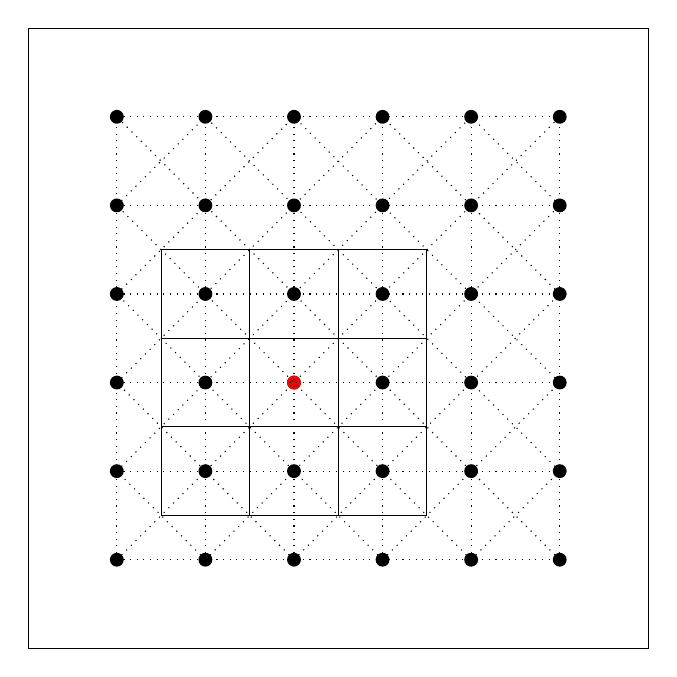
\begin{tikzpicture}[scale=1.125]%[scale=0.75]
        \tikzstyle{every node}= [circle,fill=black, minimum size= 5pt,inner sep=0pt];
          \foreach \x in {1,2,3,4,5,6}{
            \foreach \y in {1,2,3,4,5,6}{
              \node(\x\y) at (\x,\y) {};
            }
          }
          \node(33)[circle,fill=red] at (3,3) {};
          \foreach \x in {1.5,2.5,3.5,4.5}{
            \path[thin]
            (\x,1.5) edge (\x,4.5)
            (1.5,\x) edge (4.5,\x);
          }

          %\draw[ultra thin] (1,6.17) edge[<->] (2,6.17);
          %\node[draw=none,fill=none] at (1.5,6.3) {\scriptsize{$\mu$}};

          \foreach \x in {1,2,3,4,5,6}{
            \draw[dotted,thin] (1,\x) -- (6,\x);
            \draw[dotted,thin] (\x,1) -- (\x,6);
          }

          \foreach \x in {1,2,3,4,5}{
            \draw[dotted,thin] (1,\x) -- (7-\x,6);
            \draw[dotted,thin] (6,\x) -- (\x,6);
          }

          \foreach \x in {2,3,4,5}{
            \draw[dotted,thin] (\x,1) -- (6,7-\x);
            \draw[dotted,thin] (7-\x,1) -- (1,7-\x);
          }

          \draw (0,0) rectangle (7,7);

          %\node[draw=none,fill=none] at (0.9,0.4) {$S=\bbe$};
      \end{tikzpicture}
      \caption{Weight assignement of convolutions on pixel domains}
      \label{fig:rect}
\end{figure}